\documentclass[a4paper,11pt]{article}
\usepackage{fullpage}
\voffset=10mm
\hoffset=-3mm

\usepackage{cite}
\usepackage{multirow}
\usepackage{graphicx}
\usepackage{url}
\usepackage{xspace}

\def\gled{\textsc{Gled}\xspace}
\def\p7{\textsc{Project7}\xspace}
\def\grid{\texttt{grid}\xspace}
\def\smalltt#1{{\small\texttt{#1}}}
\def\foottt#1{{\footnotesize\texttt{#1}}}

%\looseness=-1 end slimy pars with this

\title{Authentication \& Authorization Infrastructure of \gled}
\author{Matev\v{z} Tadel}

\begin{document}

\maketitle

\begin{abstract}
  This document describes implementation-level details of
  authentication and authorization mechanisms of the \gled framework.
\end{abstract}

\pagestyle{myheadings}
\thispagestyle{plain}
\markboth{}{Authentication \& Authorization Infrastructure of \gled}

%%%%%%%%%%%%%%%%%%%%%%%%%%%%%%%%%%%%%%%%%%%%%%%%%%%%%%%%%%%%%%%%%%%%%%%%

\section{Introduction}

The main function of the \gled system is to allow collaborative access
to object collections distributed across a hierarchic structure
of computing nodes. Each node can maintain its own object collections
and can export them to nodes on the next (lower) level of the
hierarchy.

Upon receiving the mirroring request the higher node sends a
data-stream to the new connecter that allows construction of the
mirror image on the client side.  After the initial mirroring the
consistency of the object collection is maintained via time-ordered
delivery of \emph{method invocation requests} (MIR). MIR is, in its
essence, nothing but a message that can be unambiguously interpreted
in a context of an object graph and results in an invocation of a
method (with well-defined arguments and arbitrary data-stream attached
at its end) in a given object.

All changes of the object graph and all state changes of
individual objects are representable by MIRs. A change can be
algorithmic (the execution of the method results in a change of the
object state) or the method call can contain further data that will
replace part of object's data (e.g. \emph{set} methods). If the change
is algorithmic, it can be performed at all nodes and thus a balancing
between network bandwidth usage and node CPU usage can be achieved.

Sources of MIRs are servers/proxies/clients (Saturns) running at
computing nodes connected into the hierarchy and viewers (Eyes)
connected to the nodes. Saturns and Eyes are represented as \gled
objects in the object collection of the top-level server and therefore
the cluster structure is known to all nodes. Sender of each MIR can
be identified by the \gled object that represents the Saturn or Eye.

The details of the core \gled system are described in \cite{gled-1}.
The terminology used in the rest of this paper is also described there
(a short vocabulary is given in App.\,\ref{app:gled-terminology}).

%%%%%%%%%%%%%%%%%%%%%%%%%%%%%%%%%%%%%%%%%%%%%%%%%%%%%%%%%%%%%%%%%%%%%%%%

\section{Overview}

The basic idea of any authentication \& authorization scheme is to
identify the sender of a request for certain action and to determine
if the sender is authorized to perform it. In \gled the authentication
is performed during connection of a new Saturn (client/proxy) or Eye
(viewer). The authorization is performed during \emph{blessing} of a
MIR by a queen.\footnote{Flares (broadcasted MIRs) are blessed only on
  the Saturn that holds target of the MIR in its sun-space. Beams
  (directed MIRs) are blessed on the executing Saturn irrespective of
  the source or target of the MIR.} %
The MIR structure contains the identification of the caller and thus
the authorization problem becomes: ``Is the caller allowed to execute
this particular MIR?''

Direct method calls made during execution of MIRs or threads are not
subjected to any kind of authorization procedure. This is a design
decision that allows complex operations to be performed swiftly. On
the other hand, MIRs emitted during execution of a MIR or a thread are
considered to be emitted by the same entity that emitted the MIR or
started the thread. This behaviour is enforced at the level of Saturn
(server/proxy/client and MIR router) and Mountain (thread manager).

There are three base glasses that form the core of \gled's A\&A
infrastructure:
\begin{enumerate}

\item \texttt{ZIdentity}: lenses of this glass are mostly static and
  represent identities in the context of a \gled cluster. Group
  identities are represented by \smalltt{ZGroupIdentity} glass. It
  contains a list of basic identities that are actively using this
  group identity.
  
\item \texttt{ZMirEmittingEntity} (MEE): sub-glasses of this glass represent
  Saturns (\smalltt{SaturnInfo}) and Eyes (\smalltt{EyeInfo}) connected
  into the cluster. A MIR emitting entity has a \emph{primary
    identity} and a list of \emph{active identities} that can change
  dynamically.

  Authentication is the procedure of establishing the link between a
  \texttt{MirEmittingEntity} and its primary \smalltt{ZIdentity}.
  
\item \texttt{ZMirFilter} is the base glass for authorization modules.
  Sub-glasses contain further data that determines the interrogative
  procedure for each MIR passing through the filter. The
  \smalltt{ZFilterAggregator} filter allows stacking of several filters
  into a list and can be used to set-up arbitrarily complex
  authorization conditions.
  
  The most obvious MIR filters are based on identity of the caller
  (\texttt{ZIdentityFilter} and \smalltt{ZIdentityListFilter}) and
  provide \emph{access list} implementation.

\end{enumerate}

Now the basic elements of authorization infrastructure are in place.
But nothing has been said about how they are connected into the object
structure and how they are assigned to individual lenses or their
collections.

First it is important to note that all elements (identities, MEEs and
filters) are represented as \gled classes (glasses) and can thus be
created and manipulated by using the standard \gled mechanisms. Hence
they can be easily instantiated, replicated and modified in a cluster
context. But what is particularly important: they can be referenced by
any lens via either object-aggregation method of \gled, i.e. they can
be linked to and contained in lists.

Each lens can be protected individually by its own MIR filter (named
\emph{guard}). Several lenses can have the same access restrictions by
simply referencing the same filter.

Further, each queen has an additional guard (called \emph{protector})
that guards all queen's subjects.\footnote{The \foottt{ZQueen} glass is in
  charge of instantiation and deletion of objects in its object-space
  called the \emph{queen-space}. The queen-space is the smallest chunk
  of Saturn's object space that can be mirrored independently.} %
The authorization procedure performed during
blessing of a MIR (in method \smalltt{ZQueen::\-BlessMIR(ZMIR\&)}) can be
configured via other data members of the \smalltt{ZQueen} to take
either or both of the guards into account. The details of MIR
filtering and blessing are described in Sec.\,\ref{sec:Authorization}.

\begin{figure}[tb]
\centering
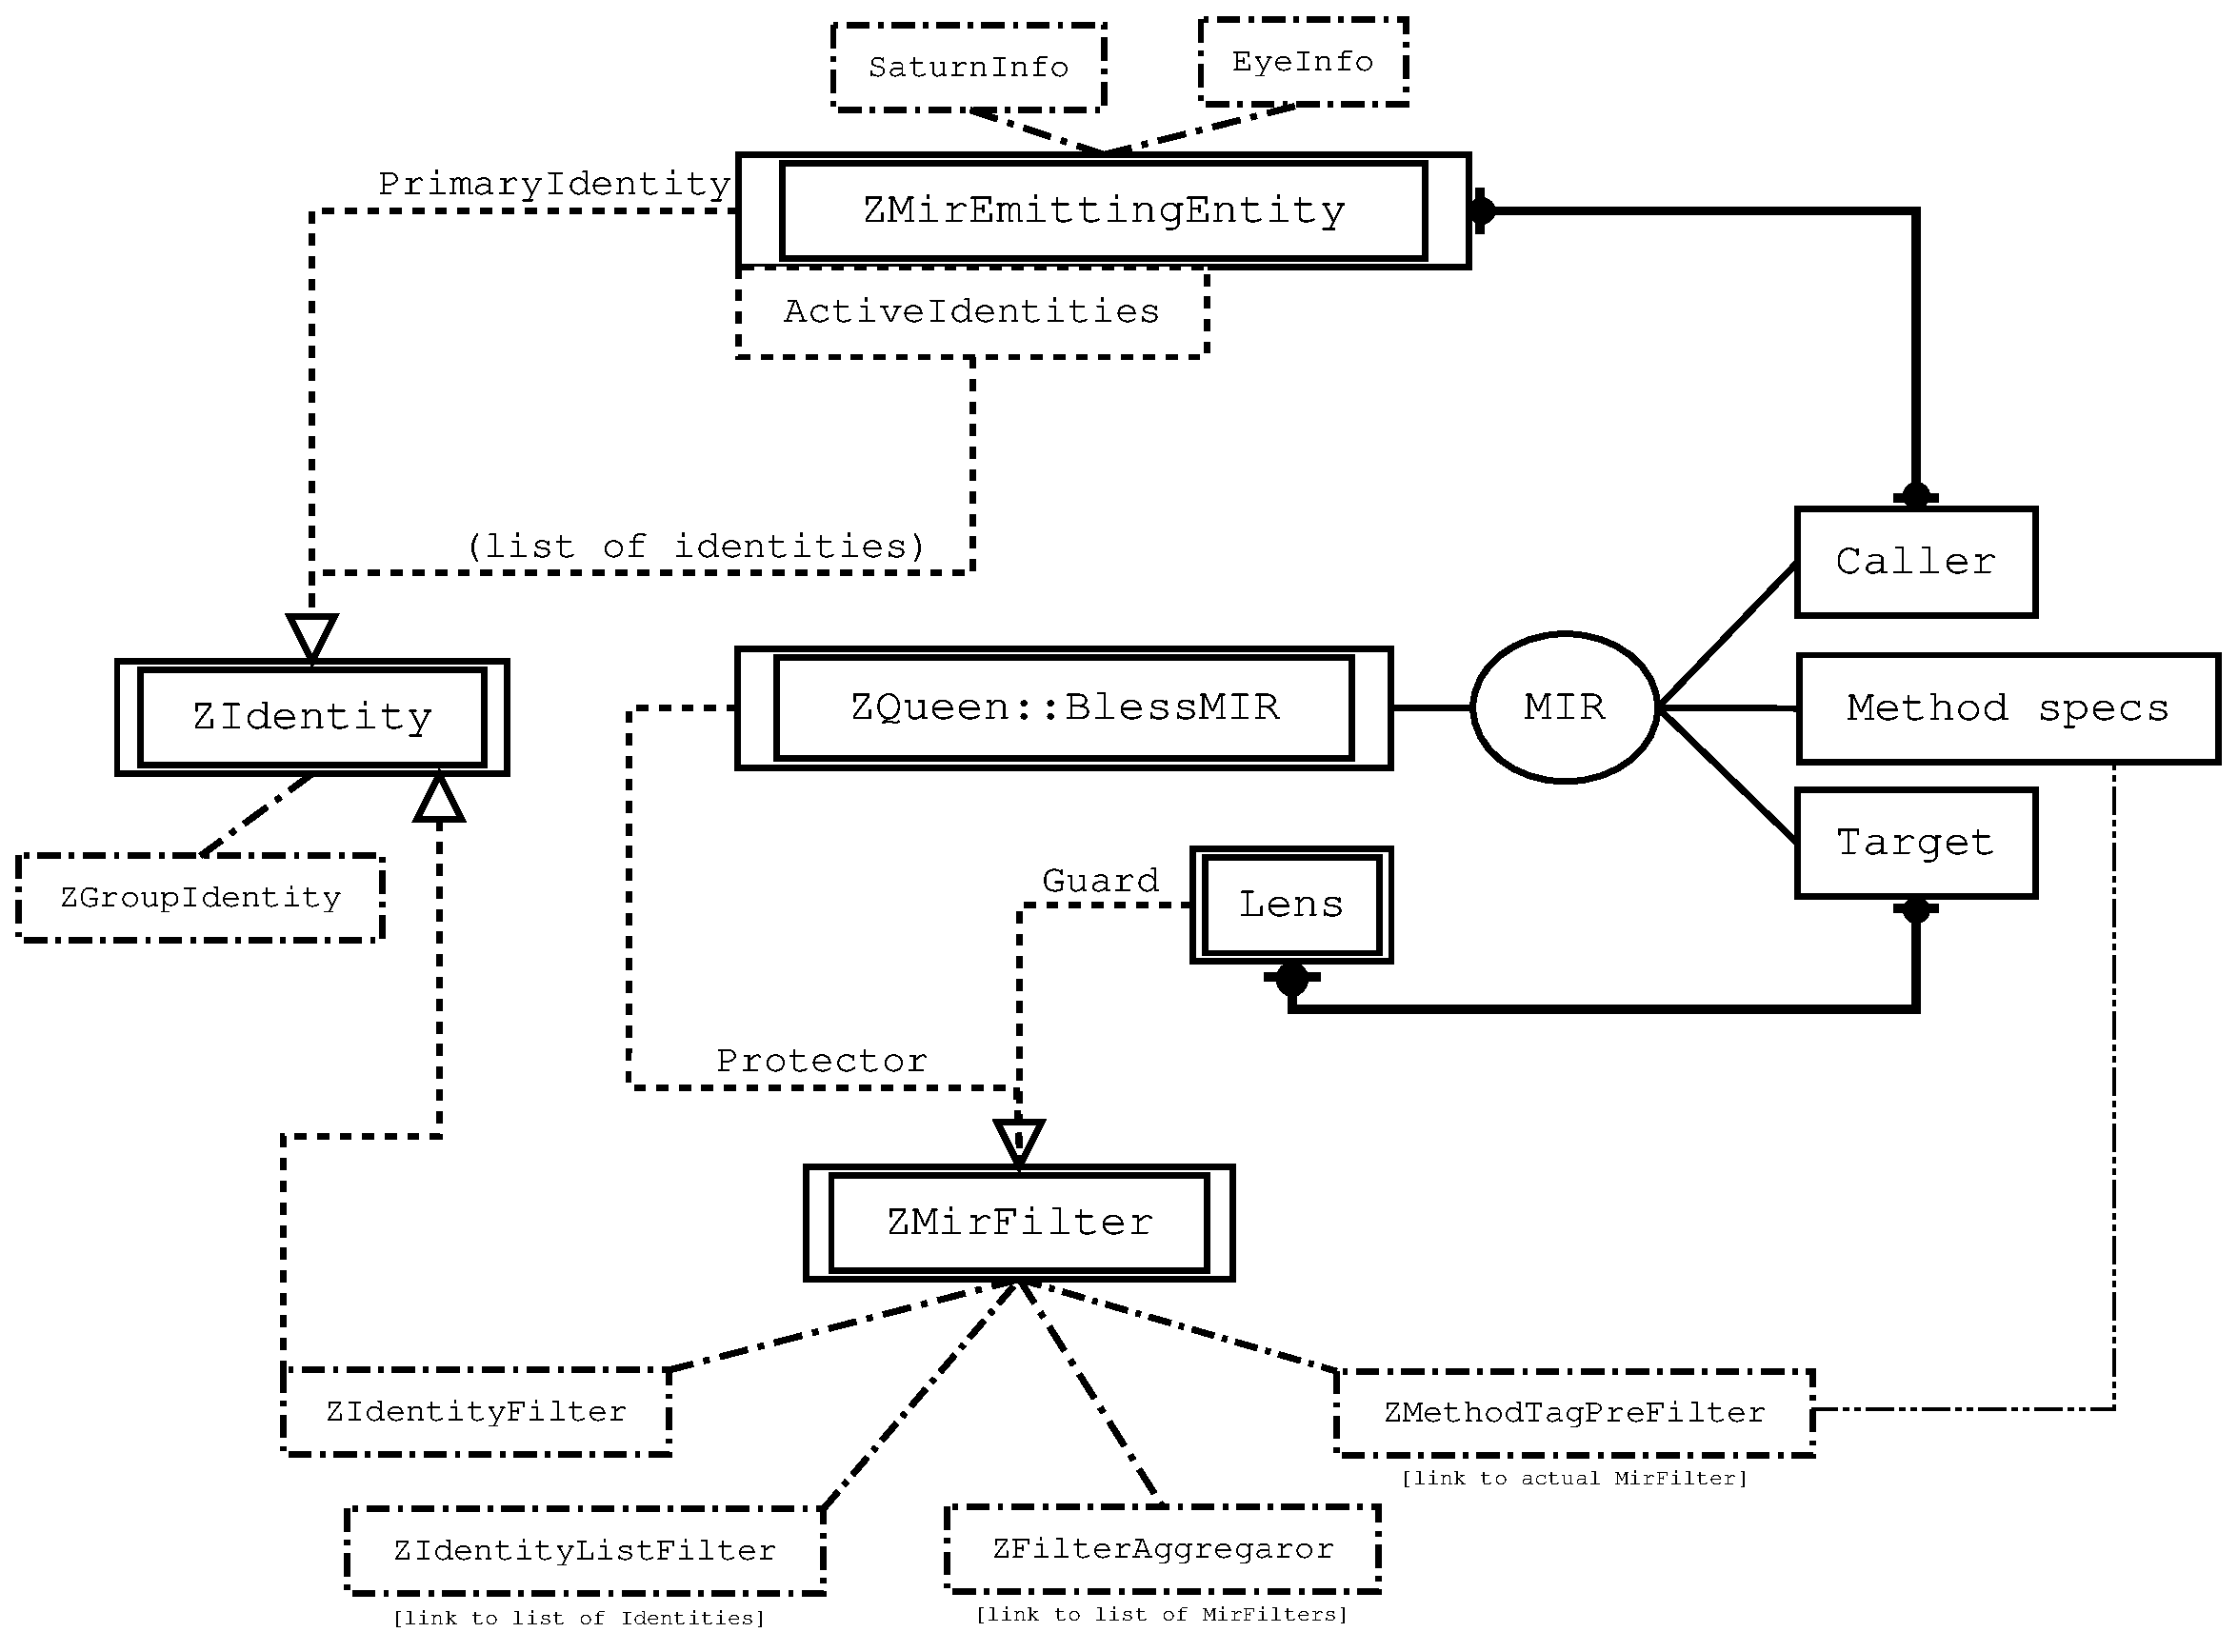
\includegraphics[width=\textwidth]{aa_elements}
\caption{}
\label{fig:AA_elements}
\end{figure}


There is no explicit concept of a user in the presented A\&A scheme.
In fact it has been split into two concepts: the \emph{connection}
(\smalltt{ZMirEmittingEntity}) and the \emph{identity}
(\smalltt{ZIdentity}). This allows a MEE to simultaneously wield
several identities as well as to dynamically change the list of active
identities. The identity can be naturally extended to a \emph{group
  identity} which can effectively be mapped to a list of identities
that can request the activation of the group identity in a context
of a given MEE. The user as a factually existing entity can be
reestablished as a link between a MEE and its primary identity.


\textbf{Accounting} could be implemented by extending the queen class
with logging facilities. Further, some central mechanism should also
be provided on the Saturn level as there can be any number of queens 
ruling on each Saturn.

%%%%%%%%%%%%%%%%%%%%%%%%%%%%%%%%%%%%%%%%%%%%%%%%%%%%%%%%%%%%%%%%%%%%%%%%

\section{Authentication procedure}
\label{sec:Authentication}

Authentication is performed during handshake process when \gled object
representing the connection is incorporated into the object structure
representing the cluster. A successful authentication results in an
established link between a MIR-emitting entity and identity claimed by
the connection.

Current implementation of the authentication procedure is based on the
RSA public key cryptography and uses challenge-response
authentication. All further communication `trusts' the accepted socket
and is not encrypted. This requires a repository for the keys and the
built-in implementation uses a UNIX directory structure for storage of
the keys. The root of the structure is stored in the top \gled object:
\smalltt{TString Gled::mAuthDir} (it defaults to
\smalltt{ENV\{HOME\}/\-.gled/\-auth}, but can be changed with the
\smalltt{-authdir} command-line option). The keys are stored in the
\smalltt{public\_keys} and \smalltt{private\_keys} directories with
the individual filename being equal to the name of the identity it is
representing. This means that if you want to allow user
\smalltt{foo.bar@baz.org} to login to the cluster, you must obtain his
public key and copy it to the \smalltt{public\_keys} directory.  Group
membership information is stored in the \smalltt{groups} directory.
Each group is represented by a file (again, with the same name as the
group) which is simply a new-line separated list of identities that
are allowed to claim this group identity. By convention the group
names begin with the \smalltt{@} character (e.g. \smalltt{@admin} or
\smalltt{@master@baz.org}).

So far no attempt was be made to provide user and group management
interfaces. In the current \gled distribution the management task
reduces to simple file-system operations and editing of files.

The authentication procedure proceeds through the following steps:
\begin{enumerate}\parsep=0pt\itemsep=0pt
  
\item The connecting MEE opens a TCP/IP socket to the server port of
  the Saturn it is attempting to connect to (${\cal S}_i$). After the
  initial handshake the MEE issues a MEE connection request
  (\smalltt{GledNS::MT\_MEE\_Connect}) accompanied by a serialized
  \smalltt{SaturnInfo} or \smalltt{EyeInfo} structure. The login
  identity must be specified by setting the
  \smalltt{ZMirEmittingEntity::mLogin} string variable. This will
  become the primary identity of the MME.

\item ${\cal S}_i$ sends a request for initiation of a new MEE
  connection to the SunAbsolute (${\cal S}_0$), again followed by the
  streamed MEE. ${\cal S}_0$ returns either the \emph{connection
    identifier} to ${\cal S}_i$ or denies the connection.
  
\item ${\cal S}_i$ forwards the connection identifier to the MEE. The
  MME then establishes a direct connection to ${\cal S}_0$ (TCP/IP
  socket) and requests authentication for the given connection
  identifier.
  
\item ${\cal S}_0$ returns the challenge string, encrypted with the
  public part of the RSA key belonging to the MME's login identity
  (note the a streamed MME has already been sent to ${\cal S}_0$ by
  ${\cal S}_i$), followed by the public key of the ${\cal S}_0$.

\item The MME decrypts the challenge using its private key,
  re-encrypts it by the public key of the ${\cal S}_0$ and sends it
  back to ${\cal S}_0$.

\item ${\cal S}_0$ decrypts the message and compares it with the
  original challenge. On success the MEE is added to the cluster and
  associated with the claimed login identity.

\end{enumerate}

\subsection{Acquiring further identities}
%%%%%%%%%%%%%%%%%%%%%%%%%%%%%%%%%%%%%%%%%
\label{ssec:Authentication_FurtherIDS}

For now, only group identities can be attached to a MME as additional
active identities. The procedure is simple: a MIR has to be sent to
the SunQueen with the aspired identity as the argument:
{\footnotesize\begin{verbatim}
ZGroupIdentity* new_identity = <sth>;
auto_ptr<ZMIR> mir( sun_queen->S_AttachIdentity(new_identity) );
mSaturn->ShootMIR(mir);
\end{verbatim}}
SunQueen performs the relevant checks and emits all necessary
MIRs. A MME can only have a single instance of any group identity
in its list of active identities.

To remove a given identity, the converse method
\smalltt{ZSunQueen::DetachIDentity(id)} must be called via a MIR.

\subsection{External identity servers}
%%%%%%%%%%%%%%%%%%%%%%%%%%%%%%%%%%%%%%

Ideally one would wish for an extension of the concept of the identity
so that further specializations could use external databases and/or
mechanisms for authentication and for resolving of group membership
queries.

%%%%%%%%%%%%%%%%%%%%%%%%%%%%%%%%%%%%%%%%%%%%%%%%%%%%%%%%%%%%%%%%%%%%%%%%

\section{Authorization procedure}
\label{sec:Authorization}

Authorization performed for MIRs. The process of blessing: dependency
check of context arguments followed by authorization.

In the context of a MIR authorization, there are two filters that
can be used in the authorization:
\begin{enumerate}

\item \emph{Guard} of the lens that will execute the MIR (or a lens
  at which the method call request is directed).

 \smalltt{class ZGlass\,\{\,ZMirFilter* mGuard;\,\};}

 With guards individual lenses can have their own access permissions.
 
\item \emph{Protector} of the queen ruling to the target lens (the
  queen that is performing the MIR blessing).

  \smalltt{class ZQueen\,\{\,ZMirFilter* mProtector;\,\};}

  Protectors serve to all lenses of a given queen (including the queen
  herself) and thus provide a method of setting access rights for a
  logical group of lenses.

\end{enumerate}

Queen has further configuration variables that fully specify in what
sequence the two filters will be used to decide the authorization
problem. The MIR filtering details are explained in
Sec.\,\ref{sec:MIR_Filters}. Any MIR filter, when presented with a
particular MIR, returns its judgment: \emph{allow}, \emph{deny} or
\emph{none}. It is important that a filter can have no particular
opinion about the MIR (indicated by the \emph{none} return value):
this allows for an easy implementation of compound filters. Further,
it makes the MIR filtering procedure symmetric with respect to the
final judgment and goal of the individual filter: it can
\emph{allow/deny} the execution \emph{if/unless} certain
conditions are met.

Consider the authorization related part of the \smalltt{ZQueen} glass:
{\footnotesize\begin{verbatim}
class ZQueen : public ZNameMap {
  ...
public:
  enum AuthMode_e { AM_None=0, AM_Queen, AM_Lens,
                    AM_QueenThenLens, AM_LensThenQueen };
  enum Align_e    { A_Good=0, A_Evil };
protected:
  UChar_t       mAuthMode;  // X{GS} 7 PhonyEnum(-vals=>[AM_Null, AM_Queen, ...])
  UChar_t       mAlignment; // X{GS} 7 PhonyEnum(-vals=>[A_Good, A_Evil])
  UChar_t       mMapNoneTo; // X{GS} 7 PhonyEnum(-vals=>[R_Allow, R_Deny])

  ZMirFilter*   mProtector; // X{GS} L{}
public:
  virtual void BlessMIR(ZMIR& mir) throw(string);
  ...
};
\end{verbatim}
}

Authentication mode (\smalltt{mAuthMode}) specifies any selection of
the two filters. If both filters are used, the order in which they
will be considered can be selected. Together with queen
\emph{alignment} this can serve for optimization of the access
checking procedure.

Alignment (\smalltt{mAlignment}) is relevant for modes that use both
filters. Good queens prefer to \emph{allow} the MIR execution. If the
first filter returns \emph{allow} they immediately allow the
execution. If the first filter returns \emph{deny}, they still
consider the second filter. And conversely for queens that have evil
alignment and prefer to \emph{deny} the execution.

Default judgment (\smalltt{mMapNoneTo}): if both filters are undecided
(or if authentication mode is set to \emph{none}) than the MIR is
blessed if it is set to \emph{allow} and discarded if it set to
\emph{deny}.  In contrast to MIR filters, a queen can not be undecided
about the fate of a particular MIR: it can either be blessed (and will
be executed) or it has to be excommunicated.

%%%%%%%%%%%%%%%%%%%%%%%%%%%%%%%%%%%%%%%%%%%%%%%%%%%%%%%%%%%%%%%%%%%%%%%%

\section{MIR Emitting Entities}

\emph{MIR emitting entities} (MEE) can emit MIRs into a \gled cluster.
To emit a MIR, it has to be made available to a Saturn which then,
depending on the type and recipient of the MIR, routes it towards it
recipient and/or executes it.

{\footnotesize\begin{verbatim}
class ZMirEmittingEntity : public ZGlass {
  ...
protected:
  TString               mLogin;                 // X{GS} 7 TextOut()
  ZIdentity*            mPrimaryIdentity;       // X{GS} L{}
  ZHashList*            mActiveIdentities;      // X{GS} L{}
public:
  Bool_t HasIdentity(ZIdentity* ident);
  ...
};
\end{verbatim}
}

Each MME has a login user name (\smalltt{mLogin}) which is, during the
authentication procedure, linked to the primary identity
(\smalltt{mPrimaryIdentity}) of the MME. Further identities can be
associated with a MME (see Sec.\,\ref{ssec:Authentication_FurtherIDS}) and they are stored
in the list pointed to by the link \smalltt{mActiveIdentities}.

The \smalltt{HasIdentity(ZIdentity* ident)} method can be used to
establish the presence of \smalltt{ident} as either the primary or any
of the active identities.

\subsection{\smalltt{SaturnInfo}}
%%%%%%%%%%%%%%%%%%%%%%%%%%%%%%%%%

Instances of the \smalltt{SaturnInfo} glass represent Saturns in a
\gled cluster. 

{\footnotesize\begin{verbatim}
class SaturnInfo : public ZMirEmittingEntity {
  ...
protected:
  Bool_t        bUseAuth;       // X{GS} 7 BoolOut()
  SaturnInfo*   mMaster;        // X{GS} L{}
  ZHashList*    mMoons;         // X{GS} L{}
  ZHashList*    mEyes;          // X{GS} L{}
  ...
};
\end{verbatim}
}

Each Saturn is connected with neighbouring Saturns in the node
hierarchy: the \smalltt{mMaster} link points to the relative server
(it is zero for SunAbsolute) and the list pointed to by the
\smalltt{mMoons} link contains clients of the Saturn. These structures
are actively used by a Saturn during routing of MIRs. All connected
viewers are stored in the list pointed to by the \smalltt{mEyes} link.
\smalltt{SaturnInfo} also contains some general information about the
computing node it is representing (architecture, CPU type and frequency,
amount of memory etc.).

Sources of MIRs carrying the signature of a given \smalltt{SaturnInfo}
are:
\begin{enumerate}\parsep=0pt\itemsep=0pt
\item the Saturn itself; these MIRs are mostly directed at the
  SunQueen of the SunAbsolute and serve the goal of changing the
  topology of the \gled cluster (addition/removal of
  Saturns and Eyes).
\item the ROOT shell; note that you must create the MIR and pass it to
  the Saturn either via posting or shooting.
\end{enumerate}


\subsection{\smalltt{EyeInfo}}
%%%%%%%%%%%%%%%%%%%%%%%%%%%%%%

Lenses of glass \smalltt{EyeInfo} represent the viewers or Eyes. 

{\footnotesize\begin{verbatim}
class EyeInfo : public ZMirEmittingEntity {
  ...
protected:
  SaturnInfo*   mMaster;        // X{GS} L{}
  ...
};
\end{verbatim}
}

Note that Eyes have TCP/IP connection to the local Saturn and that
they are not allowed to directly manipulate the available objects. For
every user action a MIR is created and sent to the Saturn. It then
sets the caller variable of the MIR to the \smalltt{EyeInfo} structure
that represents the Eye in the cluster.

%%%%%%%%%%%%%%%%%%%%%%%%%%%%%%%%%%%%%%%%%%%%%%%%%%%%%%%%%%%%%%%%%%%%%%%%

\section{Identities}

Identities are mostly static lenses (of glass \smalltt{ZIdentity})
that serve two purposes:
\begin{enumerate}\parsep=0pt\itemsep=0pt
\item to be attached to MEEs that have proved to be worthy
\item to be referenced by MIR filters to either allow or deny certain
  action to the possessors of given identities
\end{enumerate}
The name of the lens (declared in \smalltt{class ZGlass\,\{\,TString
    mName;\,\};}) is reused for the unique identification string of the
given identity.

{\footnotesize\begin{verbatim}
class ZIdentity : public ZGlass {
  ...
protected:
  UInt_t                mNumMMEs;       // X{GS} 7 ValOut()
  ZMirFilter*           mAllowThis;     // X{GS} L{}
  ...
};
\end{verbatim}
}

Each identity knows a number of MMEs that are using it
(\smalltt{mNumMMEs}). A default MIR filter is created and linked at
the identity instantiation time (link \smalltt{mAllowThis};
returns \emph{allow} if the calling MME has the identity and
\emph{deny} otherwise).

\subsection{\texttt{ZGroupIdentity}}
%%%%%%%%%%%%%%%%%%%%%%%%%%%%%%%%%%%%

The \texttt{ZGroupIdentity} represents a group of users.

{\footnotesize\begin{verbatim}
class ZGroupIdentity : public ZIdentity {
  ...
protected:
  ZNameMap*     mActiveMMEs;    // X{GS} L{}
  ...
};
\end{verbatim}
}

In addition to the identity the group identity also contains a link to
list of MEEs that are currently using the group as one of theirs active
identities.

%%%%%%%%%%%%%%%%%%%%%%%%%%%%%%%%%%%%%%%%%%%%%%%%%%%%%%%%%%%%%%%%%%%%%%%%

\section{MIR Filters}
\label{sec:MIR_Filters}

\subsection{\texttt{ZMirFilter}}
%%%%%%%%%%%%%%%%%%%%%%%%%%%%%%%%

\texttt{ZMirFilter} is the base class for all MIR filters.  Its
functionality is provided by a virtual method \smalltt{FilterMIR}:

{\footnotesize\begin{verbatim}
class ZMirFilter : public ZGlass {
  ...
  enum    Result_e { R_None=0x1, R_Allow=0x2, R_Deny=0x4 };
  virtual Result_e FilterMIR(ZMIR& mir);
protected:
  UChar_t mMapNoneTo; // X{GS} 7 PhonyEnum(-vals=>[R_None, R_Allow, R_Deny])
  ...
};
\end{verbatim}
}
    
A MIR filter can be \emph{undecided} about a MIR: in this case it
returns \smalltt{ZMirFilter::R\_None}. But sometimes this is
undesirable and \smalltt{R\_None} should be mapped to
\smalltt{R\_Allow} or \smalltt{R\_Deny}. That's the purpose of the
\smalltt{mMapNoneTo} data-member. As glasses always use public
inheritance from glass bases the variable is available from all
filters and can be used to tailor filter behaviour to its function.

The \smalltt{FilterMIR()} method is trivial: it returns the value of
\smalltt{mMapNoneTo}.


\subsection{Identity Filters}
%%%%%%%%%%%%%%%%%%%%%%%%%%%%%

Identity filters provide the core functionality of authorization as
in most cases it is the identity of the caller that decides if a
MIR is allowed to be executed.

\subsubsection{\texttt{ZIdentityFilter}}

{\footnotesize\begin{verbatim}
class ZIdentityFilter : public ZMirFilter {
  ...
protected:
  ZIdentity*    mIdentity;      // X{GS} L{}
  UChar_t       mOnMatch;       // X{GS} 7 PhonyEnum(-vals=>[R_Allow, R_Deny])
  ...
};
\end{verbatim}
}

The \smalltt{ZIdentityFilter} checks if the calling MEE (obtained from
\smalltt{ZMIR::Caller}) is in possesion of identity
\smalltt{mIdentity} and returns \smalltt{mOnMatch} if it is and the
negated result if it is not. If the \smalltt{mIdentity} link is not
set it returns whatever \smalltt{R\_None} maps to.

The check if MEE has a given identity is performed by calling
\smalltt{Bool\_t\- ZMirEmittingEntity::\-HasIdentity(mIdentity)}. This
method returns \emph{true} if the identity is either the primary
identity of the MEE or it exists in the list of its active identities.


\subsubsection{\texttt{ZIdentityListFilter}}

{\footnotesize\begin{verbatim}
class ZIdentityListFilter : public ZMirFilter {
  ...
protected:
  ZHashList*    mIdentities;    // X{GS} L{}
  UChar_t       mOnMatch;       // X{GS} 7 PhonyEnum(-vals=>[R_Allow, R_Deny])
  ...
};
\end{verbatim}
}

The identity list filter behaves exactly like the identity filter with
the only difference that it checks if MEE is in possesion of any identity in
the list \smalltt{mIdentities}. The check stops on first match and
\smalltt{mOnMatch} is returned.


\subsection{\texttt{ZFilterAggregator}}
%%%%%%%%%%%%%%%%%%%%%%%%%%%%%%%%%%%%%%%

Filter aggregators are the basic building block of complex
authorization checks. An aggregator holds a link to a list of
subordinate filters and traverses them in list order.

{\footnotesize\begin{verbatim}
class ZFilterAggregator : public ZMirFilter {
  ...
protected:
  Bool_t        bStrongNone;    // X{GS} 7 Bool(-join=>1)
  Bool_t        bPreemptNone;   // X{GS} 7 Bool()
  Bool_t        bPreemptAllow;  // X{GS} 7 Bool(-join=>1)
  Bool_t        bPreemptDeny;   // X{GS} 7 Bool()

  ZHashList*    mFilters;       // X{GS} L{}
  ...
};
\end{verbatim}
}

During the traversal the results returned by individual filters are
accumulated (the values of \smalltt{ZMirFilter::Result\_e} constitute
a bit field) by bitwise \emph{or} operation.

The traversal can terminate before the end of the list (preempt) if
the result returned by a filter has the corresponding preemption flag
set (members \smalltt{bPreemptXyz}). In this case the return value of
the filtering operation is the return value of the filter that caused
the preemption. The \smalltt{R\_None} value is remapped if necessary.

When the list traversal is complete\footnote{Traversal also finishes
  when both \foottt{R\_Allow} and \foottt{R\_Deny} bits are set.} %
the following logic is applied:
\begin{enumerate}\parsep=0pt\itemsep=0pt
\item if both \smalltt{R\_Allow} and \smalltt{R\_Deny} bits are set
  the remapped value of \smalltt{R\_None} is returned;
  after that step only one of the \smalltt{R\_Allow} and \smalltt{R\_Deny}
  bits can be set in the collected result, and possibly also the
  \smalltt{R\_None} bit
\item if \smalltt{R\_None} bit is set and \smalltt{bStrongNone}
  variable is \emph{true}, then a remapped \smalltt{R\_None} is returned
\item if \smalltt{R\_Allow} or \smalltt{R\_Deny} is set, it is
  returned
\item a remapped \smalltt{R\_None} is returned
\end{enumerate}

The described algorithm covers all cases when only the bitwise
\emph{or} of all the results matter. One could also implement a voting
scheme, but it somehow misses the gist of a predictable authorization
system.

Filter aggregators can of course be in the filter list and thus
arbitrarily complex filters can be constructed. As filters are
glasses, some typical compound filters can be created once and reused
by incorporating them into the object graph on several points.


\subsection{\texttt{ZMethodTagPreFilter}}
%%%%%%%%%%%%%%%%%%%%%%%%%%%%%%%%%%%%%%%%%

Exported methods (and the implicit \emph{set} methods) can have any
number of method tags (character strings) assigned to them. The tags
are declared in the header file by using the \smalltt{Tags\{<tag1>,
  <tag2>, \dots\}} syntax, recognized by the \p7 parser and inserted
into the glass catalog.\footnote{In principle method tags can also
  be edited on run-time, but there is no centrally provided mechanism
  for such operations.}

The idea of the \emph{method tag pre-filter} is that it only applies a
filter if the method being posted for execution has one of specified
tags.

{\footnotesize\begin{verbatim}
class ZMethodTagPreFilter : public ZMirFilter {
  ...
protected:
  TString       mTags;          // X{GS} 7 Textor(-width=>20)
  ZMirFilter*   mFilter;        // X{GS} L{}
  ...
};
\end{verbatim}
}

The \smalltt{mTags} member holds a comma-separated list of tags for
which the \smalltt{mFilter} will be applied. If a tag is found and the
filter is set, the result of the filter is returned. If the filter is
not set, a remapped \smalltt{R\_None} is returned. If the tag is not
found, the remapping is \textbf{not done} and \smalltt{R\_None} is
returned.

By using the method tag pre-filter, one can selectively allow or disallow
access to a specific part of the interface of a given object.

%%%%%%%%%%%%%%%%%%%%%%%%%%%%%%%%%%%%%%%%%%%%%%%%%%%%%%%%%%%%%%%%%%%%%%%%

\section{The Default Security Settings}

At the Sun start-up all user and group identities available from the
\smalltt{Gled::AuthDir} are scanned and corresponding identity objects
created as children of the SunQueen.\footnote{Other Saturns receive this
information as part of the Saturn connection protocol.} %
SunQueen (as do all queens) offer a directory structure and
Authentication and authorization related lenses are stored in the
directory \smalltt{Auth}. It contains the following standard directories:
\begin{enumerate}\parsep=0pt\itemsep=0pt
\item \texttt{Identities:} all identities found in
  \smalltt{Gled::AuthDir/public\_keys}
\item \texttt{Groups} all groups found in \smalltt{Gled::AuthDir/groups}
\item \texttt{Filters} standard filters, used to protect the ruling
  class and representatives of MMEs.
\end{enumerate}

\gled requires some standard identities for proper management of the
cluster:
\begin{itemize}\parsep=0pt\itemsep=0pt
\item \texttt{sun.absolute:} corresponds to \smalltt{root}
\item \texttt{saturn:} can accept Saturns and Eyes
\item \texttt{mercury:} can not accept further MMEs; pure worker node
\item \texttt{venus:} can only accept Eyes
\item \texttt{neptune:} can only accept Saturns; proxy and/or worker
\item \texttt{guest:} identity for guest Eyes.
\end{itemize}
These identities can be used by cluster administrators to limit
functionality of a given node to one of the described functions.

By default the login identity \emph{guest} maps to \smalltt{venus} if
the connecting MEE is a Saturn and to \smalltt{guest} if it is an Eye.

Set-up of standard identities is implemented as a CINT script located in
\smalltt{ENV\{GLEDSYS\}/\-macros/\-std\_auth.C}.

%%%%%%%%%%%%%%%%%%%%%%%%%%%%%%%%%%%%%%%%%%%%%%%%%%%%%%%%%%%%%%%%%%%%%%%%

\begin{thebibliography}{9}
\bibitem{gled-1} M.\,Tadel, \emph{\gled\ -- an Implementation of the
    Hierarchic Server-Client Model}, Parallel and Distributed
  Scientific and Engineering Computing: Practice and Experience
  (editors: Y.~Pan and L.T.~Yang), Nova Science Publishers, 2003.

  A continually updated version of the
  document is available from \url{http://www.gled.org/docs/}.

\end{thebibliography}

%%%%%%%%%%%%%%%%%%%%%%%%%%%%%%%%%%%%%%%%%%%%%%%%%%%%%%%%%%%%%%%%%%%%%%%%
% Appendix
%%%%%%%%%%%%%%%%%%%%%%%%%%%%%%%%%%%%%%%%%%%%%%%%%%%%%%%%%%%%%%%%%%%%%%%%

\appendix

\section{The \gled terminology}
\label{app:gled-terminology}

\paragraph{glass:} a fully \gled enabled class (sub-class of
\texttt{ZGlass} class). Instances of glasses are called \emph{lenses}.
They are elements of \gled's object graphs and have the following
basic properties:
\begin{itemize}\parsep=0pt\itemsep=0pt
\item can be (de)serialised in a context of an obect graph
  (\texttt{Streamer()} method auto-generated by \texttt{rootcint})
\item have methods to generate and execute MIRs (generated by \p7)
\item have auto-generated low-level GUI elements that allow editing of
  lenses in a contect of a \gled viewer called \emph{Eye} (generated
  by \p7).
\end{itemize}

\end{document}
% LocalWords:  MEE SunAbsolute MMEs ZGlass TextOut
